Om met native ontwikkeling van start te gaan zullen we eerst Android Studio moeten downloaden. 
Dit kan vanop de website \url{https://developer.android.com/studio/}

\paragraph{1. Components}
Bij het eerste scherm van het installatieprogramma is het belangrijk om ook 
\textbf{Android Virtual Device} te selecteren. Deze stelt ons in staat om de applicaties die we 
zowel voor native als cross-platform zullen ontwikkelen kunnen runnen. 

\paragraph{2. Installatie locatie}
Op het volgend scherm kiezen we de locatie waar Android Studio geïnstalleerd wordt. 
Het is aangeraden om dit niet te vervangen omdat React native gebruik maakt van de standaard 
locatie om bepaalde componenten op te zoeken. 

\paragraph{3. Startmenu map}
Deze is zelf te kiezen. Hiermee creëer je een shortcut vanwaar Android Studio kan worden opgestart.

\paragraph{4. Android SDK}\label{par:sdk}
Als de installatie goed is verlopen krijgen we volgend welkom scherm te zien. 
\begin{figure}[H]
    \centering
    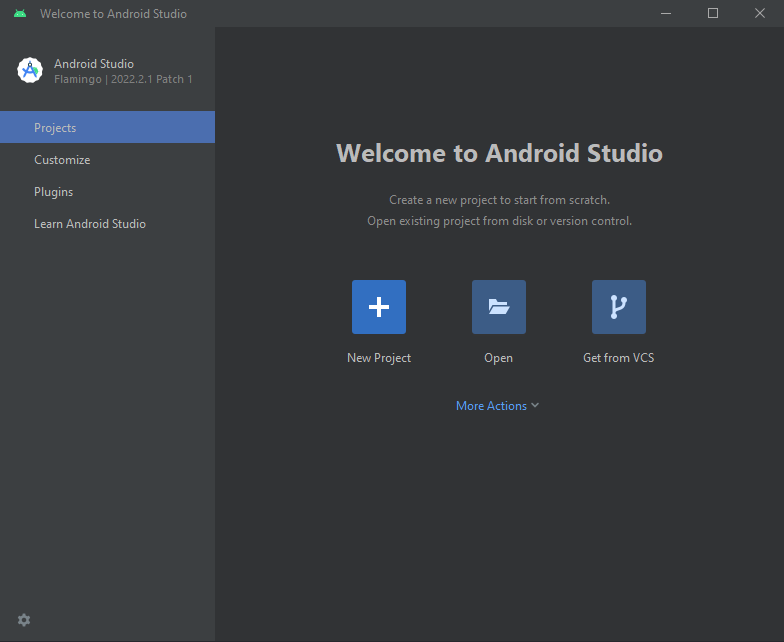
\includegraphics[height=0.4\textheight]{androidinstallatie.png}
    \caption{Startscherm na Android Studio installatie.}
\end{figure}
Standaard wordt de laatste \gls{AndroidSDK} geïnstalleerd door Android Studio. 
Deze zullen we ook tijdens de duratie van het onderzoek gebruiken. 
Maar om met deze laatste Android SDK te werken hebben we Android 13 (Tiramisu) nodig. 
Om deze te installeren drukken we op \textit{More Actions}. Op het nieuwe verkregen scherm 
kunnen we dan Android 13 (Tiramisu) aanvinken. Ook zullen we onderaan rechts het vakje 
\textbf{Show Package Details} aanvinken om dan te verifiëren dat ook zeker 
\textbf{Android SDK Platform 33}, \textbf{Sources for Android 33} en 
\textbf{Google APIs Intel x86\_64 Atom System Image} zijn aangevinkt.
\\\\
Daarna navigeren we naar SDK Tools en vinken we opnieuw \textbf{Show Package Details} 
aan en vinken we ook onder Android SDK Build-Tools \textbf{33.0.0} aan. 
Tot slot drukken we op \textbf{Apply} om de Android SDK en gerelateerde tools te downloaden en installeren. 
Maak daarna ook een dummy project aan (Empty Activity) om Android Studio van start te krijgen.

\paragraph{5. Emulator}
Om de applicaties die we zullen ontwikkelen te runnen hebben we een emulator nodig. 
Deze kunnen we aanmaken bovenaan rechts \textit{Device Manager > Create device}. 
Eerst en vooral selecteren we de device dat we willen emuleren. Voor het onderzoek 
gaan we gebruik maken van een Pixel 3 als device. Na het selecteren van ons device moeten we 
de Android versie klikken. Hier selecteren we Tiramisu met API Level 33 (Die we daarnet hebben geïnstalleerd). 
Tot slot zijn er nog een aantal configuratie instellingen voor het apparaat. Wij laten deze allemaal op hun standaard 
waarden staan.
\\\\
Nu is Android Studio klaar om native applicaties te ontwikkelen en runnen. 
